\documentclass[]{article}
\usepackage{lmodern}
\usepackage{amssymb,amsmath}
\usepackage{ifxetex,ifluatex}
\usepackage{fixltx2e} % provides \textsubscript
\ifnum 0\ifxetex 1\fi\ifluatex 1\fi=0 % if pdftex
  \usepackage[T1]{fontenc}
  \usepackage[utf8]{inputenc}
\else % if luatex or xelatex
  \ifxetex
    \usepackage{mathspec}
  \else
    \usepackage{fontspec}
  \fi
  \defaultfontfeatures{Ligatures=TeX,Scale=MatchLowercase}
\fi
% use upquote if available, for straight quotes in verbatim environments
\IfFileExists{upquote.sty}{\usepackage{upquote}}{}
% use microtype if available
\IfFileExists{microtype.sty}{%
\usepackage{microtype}
\UseMicrotypeSet[protrusion]{basicmath} % disable protrusion for tt fonts
}{}
\usepackage[margin=1in]{geometry}
\usepackage{hyperref}
\hypersetup{unicode=true,
            pdftitle={Outline of eDiscovery paper},
            pdfauthor={Richard Careaga},
            pdfborder={0 0 0},
            breaklinks=true}
\urlstyle{same}  % don't use monospace font for urls
\usepackage{color}
\usepackage{fancyvrb}
\newcommand{\VerbBar}{|}
\newcommand{\VERB}{\Verb[commandchars=\\\{\}]}
\DefineVerbatimEnvironment{Highlighting}{Verbatim}{commandchars=\\\{\}}
% Add ',fontsize=\small' for more characters per line
\usepackage{framed}
\definecolor{shadecolor}{RGB}{248,248,248}
\newenvironment{Shaded}{\begin{snugshade}}{\end{snugshade}}
\newcommand{\AlertTok}[1]{\textcolor[rgb]{0.94,0.16,0.16}{#1}}
\newcommand{\AnnotationTok}[1]{\textcolor[rgb]{0.56,0.35,0.01}{\textbf{\textit{#1}}}}
\newcommand{\AttributeTok}[1]{\textcolor[rgb]{0.77,0.63,0.00}{#1}}
\newcommand{\BaseNTok}[1]{\textcolor[rgb]{0.00,0.00,0.81}{#1}}
\newcommand{\BuiltInTok}[1]{#1}
\newcommand{\CharTok}[1]{\textcolor[rgb]{0.31,0.60,0.02}{#1}}
\newcommand{\CommentTok}[1]{\textcolor[rgb]{0.56,0.35,0.01}{\textit{#1}}}
\newcommand{\CommentVarTok}[1]{\textcolor[rgb]{0.56,0.35,0.01}{\textbf{\textit{#1}}}}
\newcommand{\ConstantTok}[1]{\textcolor[rgb]{0.00,0.00,0.00}{#1}}
\newcommand{\ControlFlowTok}[1]{\textcolor[rgb]{0.13,0.29,0.53}{\textbf{#1}}}
\newcommand{\DataTypeTok}[1]{\textcolor[rgb]{0.13,0.29,0.53}{#1}}
\newcommand{\DecValTok}[1]{\textcolor[rgb]{0.00,0.00,0.81}{#1}}
\newcommand{\DocumentationTok}[1]{\textcolor[rgb]{0.56,0.35,0.01}{\textbf{\textit{#1}}}}
\newcommand{\ErrorTok}[1]{\textcolor[rgb]{0.64,0.00,0.00}{\textbf{#1}}}
\newcommand{\ExtensionTok}[1]{#1}
\newcommand{\FloatTok}[1]{\textcolor[rgb]{0.00,0.00,0.81}{#1}}
\newcommand{\FunctionTok}[1]{\textcolor[rgb]{0.00,0.00,0.00}{#1}}
\newcommand{\ImportTok}[1]{#1}
\newcommand{\InformationTok}[1]{\textcolor[rgb]{0.56,0.35,0.01}{\textbf{\textit{#1}}}}
\newcommand{\KeywordTok}[1]{\textcolor[rgb]{0.13,0.29,0.53}{\textbf{#1}}}
\newcommand{\NormalTok}[1]{#1}
\newcommand{\OperatorTok}[1]{\textcolor[rgb]{0.81,0.36,0.00}{\textbf{#1}}}
\newcommand{\OtherTok}[1]{\textcolor[rgb]{0.56,0.35,0.01}{#1}}
\newcommand{\PreprocessorTok}[1]{\textcolor[rgb]{0.56,0.35,0.01}{\textit{#1}}}
\newcommand{\RegionMarkerTok}[1]{#1}
\newcommand{\SpecialCharTok}[1]{\textcolor[rgb]{0.00,0.00,0.00}{#1}}
\newcommand{\SpecialStringTok}[1]{\textcolor[rgb]{0.31,0.60,0.02}{#1}}
\newcommand{\StringTok}[1]{\textcolor[rgb]{0.31,0.60,0.02}{#1}}
\newcommand{\VariableTok}[1]{\textcolor[rgb]{0.00,0.00,0.00}{#1}}
\newcommand{\VerbatimStringTok}[1]{\textcolor[rgb]{0.31,0.60,0.02}{#1}}
\newcommand{\WarningTok}[1]{\textcolor[rgb]{0.56,0.35,0.01}{\textbf{\textit{#1}}}}
\usepackage{graphicx,grffile}
\makeatletter
\def\maxwidth{\ifdim\Gin@nat@width>\linewidth\linewidth\else\Gin@nat@width\fi}
\def\maxheight{\ifdim\Gin@nat@height>\textheight\textheight\else\Gin@nat@height\fi}
\makeatother
% Scale images if necessary, so that they will not overflow the page
% margins by default, and it is still possible to overwrite the defaults
% using explicit options in \includegraphics[width, height, ...]{}
\setkeys{Gin}{width=\maxwidth,height=\maxheight,keepaspectratio}
\IfFileExists{parskip.sty}{%
\usepackage{parskip}
}{% else
\setlength{\parindent}{0pt}
\setlength{\parskip}{6pt plus 2pt minus 1pt}
}
\setlength{\emergencystretch}{3em}  % prevent overfull lines
\providecommand{\tightlist}{%
  \setlength{\itemsep}{0pt}\setlength{\parskip}{0pt}}
\setcounter{secnumdepth}{0}
% Redefines (sub)paragraphs to behave more like sections
\ifx\paragraph\undefined\else
\let\oldparagraph\paragraph
\renewcommand{\paragraph}[1]{\oldparagraph{#1}\mbox{}}
\fi
\ifx\subparagraph\undefined\else
\let\oldsubparagraph\subparagraph
\renewcommand{\subparagraph}[1]{\oldsubparagraph{#1}\mbox{}}
\fi

%%% Use protect on footnotes to avoid problems with footnotes in titles
\let\rmarkdownfootnote\footnote%
\def\footnote{\protect\rmarkdownfootnote}

%%% Change title format to be more compact
\usepackage{titling}

% Create subtitle command for use in maketitle
\newcommand{\subtitle}[1]{
  \posttitle{
    \begin{center}\large#1\end{center}
    }
}

\setlength{\droptitle}{-2em}

  \title{Outline of eDiscovery paper}
    \pretitle{\vspace{\droptitle}\centering\huge}
  \posttitle{\par}
    \author{Richard Careaga}
    \preauthor{\centering\large\emph}
  \postauthor{\par}
      \predate{\centering\large\emph}
  \postdate{\par}
    \date{February 8, 2019}

\usepackage{fancyvrb}
\usepackage{hyperref}
\usepackage{graphicx}

\begin{document}
\maketitle

\begin{Shaded}
\begin{Highlighting}[]
\KeywordTok{library}\NormalTok{(pdftools)}
\KeywordTok{library}\NormalTok{(tidytext)}
\KeywordTok{library}\NormalTok{(tidyverse)}
\end{Highlighting}
\end{Shaded}

\begin{verbatim}
## -- Attaching packages ------------------------------------------------- tidyverse 1.2.1 --
\end{verbatim}

\begin{verbatim}
## v ggplot2 3.1.0       v purrr   0.3.0  
## v tibble  2.0.1       v dplyr   0.8.0.1
## v tidyr   0.8.2       v stringr 1.4.0  
## v readr   1.3.1       v forcats 0.3.0
\end{verbatim}

\begin{verbatim}
## -- Conflicts ---------------------------------------------------- tidyverse_conflicts() --
## x dplyr::filter() masks stats::filter()
## x dplyr::lag()    masks stats::lag()
\end{verbatim}

\begin{Shaded}
\begin{Highlighting}[]
\KeywordTok{library}\NormalTok{(magrittr)}
\end{Highlighting}
\end{Shaded}

\begin{verbatim}
## 
## Attaching package: 'magrittr'
\end{verbatim}

\begin{verbatim}
## The following object is masked from 'package:purrr':
## 
##     set_names
\end{verbatim}

\begin{verbatim}
## The following object is masked from 'package:tidyr':
## 
##     extract
\end{verbatim}

\hypertarget{introduction}{%
\section{Introduction}\label{introduction}}

\hypertarget{goal}{%
\subsection{Goal}\label{goal}}

The goal of this paper is to illustrate a combination of machine
learning, natural language processing and graph analysis techniques
applied to corporate email to identify potential witnessess in
litigation.

\hypertarget{background}{%
\section{Background}\label{background}}

\begin{quote}
In times of political turmoil, events can move from impossible to
inevitable without even passing through improbable.
\end{quote}

\href{https://www.project-syndicate.org/commentary/canceling-brexit-becoming-inevitable-by-anatole-kaletsky-2018-12}{Anatole
Kalesky}

\href{https://en.wikipedia.org/wiki/Enron}{Enron Corp.} and its
affiliates were engaged in energy-related businesses, as described in
its
\href{https://www.sec.gov/Archives/edgar/data/1024401/000102440101500010/ene10-k.txt}{Annual
Report on Form 10-K for the year ended December 31, 2000}

\begin{Verbatim}[frame=single]

*    the transportation of natural gas through pipelines to
markets throughout the United States;

*    the generation, transmission and distribution of
electricity to markets in the northwestern United States;

*    the marketing of natural gas, electricity and other
commodities and related risk management and finance services
worldwide;

*    the development, construction and operation of power
plants, pipelines and other energy related assets worldwide;

*    the delivery and management of energy commodities and
capabilities to end-use retail customers in the industrial
and commercial business sectors; and

*    the development of an intelligent network platform to
provide bandwidth management services and the delivery of
high bandwidth communication applications.

As of December 31, 2000, Enron employed approximately
20,600 persons.

    \end{Verbatim}

For that year it had operating revenues of \$100,789 million, according
to the same report.

On December 2, 2001, Enron filed for
\href{https://www.sec.gov/Archives/edgar/data/1024401/000102440101500046/ene8-k1214.txt}{bankruptcy
protection}.

In less than a year, Enron underwent a complete reversal of fortune as
its business strategies ran afoul of applicable regulations. The Federal
Energy Regulatory Commission (\textbf{FERC}) was one of those
regulators.

FERC
\href{https://www.ferc.gov/industries/electric/indus-act/wec/chron/chronology.pdf}{became
aware} of irregularities in the California wholesale electricity market
prices. An orientation to the issues is provided by the
\href{https://web.stanford.edu/group/fwolak/cgi-bin/sites/default/files/files/2002,\%20May\%2015_Senate\%20Committee\%20on\%20Commerce,\%20Science\%20and\%20Transportation_Wolak.pdf}{testimony}
before FERC provides a concise summary.\footnote{The short version,
  which I can relate as a former California regulatory official from
  personal knowledge, is that public electric utilities were losing a
  large share of industrial customer to self-generation. Many businesses
  found it cheaper to generate on than to pay tariff rates. Foreseeably,
  residential and business customers without the option to self-generate
  would bear the entire cost of utility fixed assets, and rates would
  increase. The solution was to require the utilities to sell their
  generation plants and buy power on a new public market on a
  ``day-ahead'' basis, tomorrow's estimated demand. Although much
  thought was devoted to the dangers of participants gaming the system
  to sell or buy at discounts for market, insuffient consideration was
  given to multi-participant cooperation.}

Following Enron's bankruptcy, FERC began an intense investigation,
including the email records of 149 Enron employees. A preliminary
\href{http://elibrary.ferc.gov/idmws/common/opennat.asp?fileID=9548231}{staff
report} issued six months later.

\hypertarget{motivating-data}{%
\subsection{Motivating Data}\label{motivating-data}}

FERC obtained approximately 500,000 emails. Copies of these were
acquired by Leslie Kaelbling of MIT and
\href{https://www.cs.cmu.edu/~./enron/}{published} by William W. Cohen
of Carnegie Mellon University. It is one of the largest publicly
available datasets of corporate email and is referred to as the Enron
Corpus. The term \emph{corpus} is used in natural language processing to
denote a collection of related text. state. It was not uncommon, for
example, for paper copies of email to be offered. These would typically
be read by teams of freelance attorneys looking for keywords. Advanced
technology included scanning with optical character recognition and some
proprietary software options to organize emails and capture the status
of review.

At the time, electronic record examination (\emph{ediscovery}) in
litigation was in a primative state. Much of the focus was directed to
keyword searches, sometimes called the \emph{smoking gun} approach.
Brute force examination misses opportunities to understand the social
networks that reflect how the organization operates, what their concerns
are and which part of the corpus should receive priority. To do that the
corpus must be distilled and analyzed.

\hypertarget{analysis}{%
\section{Analysis}\label{analysis}}

\hypertarget{data-acquisition}{%
\subsection{Data acquisition}\label{data-acquisition}}

I obtained a copy of the \href{https://www.cs.cmu.edu/~./enron/}{2009
version} of the corpus. It contains copies of emails of a private nature
that involve three users have since requested to be
\href{https://www.cs.cmu.edu/~./enron/DELETIONS.txt}{redacted}. I have
removed those 27 emails.\footnote{Most of my work on data wrangling and
  preliminary took place in 2018 in Python, relying heavily on the NLTK
  and networkx packages.}

\hypertarget{conversion}{%
\subsubsection{Conversion}\label{conversion}}

Each email was a plaintext file\footnote{Most had been generated by
  Microsoft Outlook, but some older emails were producted in IBM Notes,
  which created some character encoding issues.} Each user had a
directory tree similar to the one below.\footnote{This user had 10
  directories with 3048 files (the directory tree has been pruned to
  omit spurious detail) containing 12,147 lines and 69,226 words.}

\begin{figure}
\centering
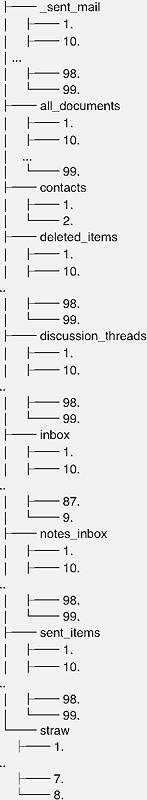
\includegraphics{https://s3-us-west-2.amazonaws.com/dslabs.nostromo/dtree.jpg}
\caption{Typical user data tree}
\end{figure}

While tedious, traversing the directory tree, parsing the emails and
loading them into an SQL database, was accomplished with a combination
of Python and Perl scripting and standard bash tools. I do not reproduce
that process here as it has little bearing on the main topic of this
paper.

\hypertarget{data-structure}{%
\subsubsection{Data structure}\label{data-structure}}

While the emails were not in native format, the plain text versions
contained nine principal segments, as shown in the figure below

Of those, the following were extracted from my earlier analysis for this
paper:

\begin{itemize}
\tightlist
\item
  sender
\item
  date
\item
  recipient
\item
  content
\end{itemize}

\hypertarget{deduplication}{%
\subsubsection{Deduplication}\label{deduplication}}

Using scripting tools, each text file extraction created a ``payload''
of the original content in the related email, capturing the text between
the beginning metadata and the following metadata for email purposes. A
payload field hash, an \href{https://en.wikipedia.org/wiki/MD5}{md5}
encoded message digest{[}\^{}In theory, it is possible that two
non-identical sequences of bytes be encoded identically, the probability
is low enough to make an md5 digest usable as a checksum verification,
its purpose here.{]} was used in the initial analysis as a primary key
to assure the uniqueness of each record. Approximately half of the
corpus consisted of duplicates, such as the original message in the
sender's sent file and one or more copies in the recipient's inbox, at a
minimum. Multiple recipients and recipients who used email folders as a
filing system were another source of duplicate messages.

\hypertarget{text-isolation}{%
\subsubsection{Text isolation}\label{text-isolation}}

For natural language processing (\textbf{NLP}) purposes, treating the
\texttt{payload} rather than the \texttt{body} as the unit of analysis
avoided an ``echo chamber'' effect of threads quoting and requoting the
original message, multipling the frequency of the words it contained.

\hypertarget{prioritization}{%
\subsubsection{Prioritization}\label{prioritization}}

Traditional analysis of emails was conducted on the principe that
``something may be overlooked,'' which delays the value of email in
preliminary analysis. Prioritizing always leaves open the option of
reviewing the set-asides later.

The first filter applied was to eliminate all email from external
addresses that were not also recipients from internal addresses. Spam,
newsletters and the like have low information potential. This filter
reduced the remaining half of the corpus by half again, leaving
approximately 125,000 emails.

A second filter for internal email was used to eliminate broadcast
messages and high frequency administrative messages. Indicia of
broadcast messages were large numbers of recipients, high frequency,
paucity of return correspondence and keyword in context screening.
Administrative messages to single recipients were identified by
frequency, lack of return correspondence and high frequency words. Many
of these were nagging emails concerning the lack of approval of expense
reports, for example. This filter reduced the dataset to approximately
24,000.

The third filter limited the dataset to emails sent before Enron's
December 2, 2001 bankruptcy. This filter reduced the email count to
approximately 13,500, about 2.7\% of the original total.\footnote{\emph{Ninety
  percent of everything is crap.} Theodore Sturgeon's Revelation, made
  in a dominantly paper-based information environment. \emph{See also}
  Pareto distributions.} A few emails dated ``1979-12-31'' were reviewed
and deleted.{[}\^{}In the technology of the day, user desktop computers
relied on an internal clock powered by a battery; when the battery died,
the date reset to what the operating system, usually a varient of
Windows, considered as the beginning of time.{]}

Finally, to achieve a practicable dataset, emails were limited to single
Enron sender to Enron single recipient, reducing the dataset further, to
9,615 emails.

\hypertarget{augmentation-and-transformation}{%
\subsubsection{Augmentation and
transformation}\label{augmentation-and-transformation}}

Each unique address in the reduced dataset was assigned a userid. The
primary purpose was to facilitate graph analysis with node identifiers
of uniform length; the second, to reduce analyst bias arising from
gender stereotyping, frequency of exposure and similar subjective
pattern seeking behaviors.

The second transformation was to create an additional field with a
\texttt{corpus} object to facilitate natural language processing.

\begin{verbatim}
enron <- enron %>% mutate(edge_corp = map(payload, tm::VectorSource)
\end{verbatim}

\hypertarget{resulting-dataset}{%
\subsubsection{Resulting dataset}\label{resulting-dataset}}

For purposes of this paper, the resulting tibble has been serialized to
an \texttt{Rda}
\href{https://s3-us-west–2.amazonaws.com/dslabs.nostromo/enron.Rda}{file}
of approximately {[} {]} size, which can be brought into an \texttt{R}
session with the following

\begin{verbatim}
  # syntax to load Rda from S3
  library(tidyverse)
  con <- url("https://s3-us-west-2.amazonaws.com/dslabs.nostromo/enron.Rda")
  load(con)
  close(con)
\end{verbatim}

\hypertarget{information-sought}{%
\subsection{Information sought}\label{information-sought}}

I downloaded the {[}staff{]} report and extracted the 6-page Executive
Summary.\footnote{This could, and would have been coded in \texttt{R}
  had multiple files been required.} From this, I extracted a list of
keywords that indicated the general nature of FERC's inquiry. I
deliberately excluded the extensive detail available in the remainder of
the report, some of which may have been derived from review of the
corpus. At the beginning of most ediscovery, the parties seeking review
of electronic documents have topics in view, which the Executive Summary
provides without biasing the analysis with the results of FERC's review.

\begin{Shaded}
\begin{Highlighting}[]
\CommentTok{# tok.R use tidytext to tokenize pdf pages}



\KeywordTok{data}\NormalTok{(stop_words)}

\NormalTok{exec_summary <-}\StringTok{ }\KeywordTok{pdf_text}\NormalTok{(}\StringTok{"sources/ExecutiveSummaryAug2002Staff.pdf"}\NormalTok{)}

\NormalTok{exec_df <-}\StringTok{ }\KeywordTok{enframe}\NormalTok{(exec_summary)}

\NormalTok{exec_tok <-}\StringTok{ }\NormalTok{exec_df }\OperatorTok\StringTok{ }\KeywordTok{unnest_tokens}\NormalTok{(word,value) }\OperatorTok\StringTok{ }\KeywordTok{select}\NormalTok{(}\OperatorTok{-}\NormalTok{name)}

\NormalTok{exec_tok <-}\StringTok{ }\NormalTok{exec_tok }\OperatorTok\StringTok{ }\KeywordTok{anti_join}\NormalTok{(stop_words)}
\end{Highlighting}
\end{Shaded}

\begin{verbatim}
## Joining, by = "word"
\end{verbatim}

\begin{Shaded}
\begin{Highlighting}[]
\NormalTok{exec_tok <-}\StringTok{ }\NormalTok{exec_tok                  }\OperatorTok
\StringTok{                }\KeywordTok{filter}\NormalTok{(}\KeywordTok{str_detect}\NormalTok{(word, }\StringTok{"[:alpha:]"}\NormalTok{))}

\NormalTok{tok_count <-}\StringTok{ }\NormalTok{exec_tok }\OperatorTok\StringTok{ }\KeywordTok{count}\NormalTok{(word) }\OperatorTok
\StringTok{                }\KeywordTok{filter}\NormalTok{ (n }\OperatorTok{>}\StringTok{ }\DecValTok{4}\NormalTok{)        }\OperatorTok\StringTok{ }
\StringTok{                }\KeywordTok{arrange}\NormalTok{(}\KeywordTok{desc}\NormalTok{(n))}

\KeywordTok{ggplot}\NormalTok{(}\DataTypeTok{data =}\NormalTok{ tok_count, }\KeywordTok{aes}\NormalTok{(}\DataTypeTok{x =}\NormalTok{ word, }\DataTypeTok{y =}\NormalTok{ n)) }\OperatorTok{+}
\KeywordTok{geom_col}\NormalTok{() }\OperatorTok{+}\StringTok{ }\KeywordTok{xlab}\NormalTok{(}\StringTok{"NULL"}\NormalTok{) }\OperatorTok{+}\StringTok{ }\KeywordTok{coord_flip}\NormalTok{()}
\end{Highlighting}
\end{Shaded}

\includegraphics{outline_files/figure-latex/keywords-1.pdf}

\begin{Shaded}
\begin{Highlighting}[]
\NormalTok{target_keywords <-}\StringTok{ }\KeywordTok{c}\NormalTok{(}\StringTok{"california"}\NormalTok{, }\StringTok{"commission"}\NormalTok{, }\StringTok{"data"}\NormalTok{, }\StringTok{"delivery"}\NormalTok{, }\StringTok{"electric"}\NormalTok{, }\StringTok{"ferc"}\NormalTok{, }\StringTok{"gas"}\NormalTok{, }\StringTok{"market"}\NormalTok{, }\StringTok{"osec"}\NormalTok{, }\StringTok{"price"}\NormalTok{, }\StringTok{"receive"}\NormalTok{, }\StringTok{"refund"}\NormalTok{, }\StringTok{"regulator"}\NormalTok{, }\StringTok{"report"}\NormalTok{, }\StringTok{"spot"}\NormalTok{, }\StringTok{"strategy"}\NormalTok{, }\StringTok{"trade"}\NormalTok{, }\StringTok{"west"}\NormalTok{)}
\end{Highlighting}
\end{Shaded}

By inspection, I selected the following keyword stems:

\begin{Shaded}
\begin{Highlighting}[]
\NormalTok{tok_count}
\end{Highlighting}
\end{Shaded}

\begin{verbatim}
## # A tibble: 44 x 2
##    word           n
##    <chr>      <int>
##  1 staff         29
##  2 prices        26
##  3 enron         22
##  4 data          21
##  5 commission    17
##  6 gas           17
##  7 price         17
##  8 california    16
##  9 natural       16
## 10 spot          15
## # ... with 34 more rows
\end{verbatim}

` with the addition of the generic term \emph{regulator.}

\hypertarget{natural-language-processing}{%
\subsection{Natural language
processing}\label{natural-language-processing}}

\hypertarget{social-network-analysis}{%
\subsection{Social network analysis}\label{social-network-analysis}}

\hypertarget{identification-of-high-value-witnesses}{%
\subsection{Identification of high-value
witnesses}\label{identification-of-high-value-witnesses}}

\hypertarget{results}{%
\section{Results}\label{results}}

\hypertarget{conclusion}{%
\section{Conclusion}\label{conclusion}}

\hypertarget{credits}{%
\section{Credits}\label{credits}}


\end{document}
